\chapter{Description et Conception du rendu}


\section{Description de la stratégie de rendu d’un état}

Pour le rendu d'un état nous avons décidé de réaliser une vue isométrique 
à l'aide de la librairie SFML de notre carte générée
aléatoirement.  
\\
\\Nous découpons la scène à rendre en couches (ou « layers ») : une couche 
pour chaque hauteur de tuile (1 à 3) et une couche par personnages.
Chacunes des couches de tuile est divisé en deux : les murs et le
plafonds. Le plafond d'une couche à la priorité sur les murs de
cette même couche et une couche supérieure à priorité sur une
couche inférieure.
\\
\\Chaque couche contiendra des informations qui seront utilisées
par la libraire Sfml : un unique tileset contenant les tuiles 
(ou « tiles »), et une unique matrice avec 
la position des éléments et les coordonnées dans la texture.
\\
\\En ce qui concerne les aspects de synchronisation, nous avons 
une horloge à 60Hz qui permet l'actualisation du rendu. 
De plus, nous avons aussi les animations des personnages 
fixes qui arrivent toutes les 60ms (soit environ 17Hz).

\section{Conception Logiciel}

Le diagramme des classes UML C++ pour le rendu est visible en Figure 3.3.

On divise le Rendu en 3 classes:

\begin{itemize}
    \item \textbf{La classe TileSet:} Elle est constitué d'un constructeur où l'on précise le type (Maptile, CharaSpritesheet) pour créer un objet TileSet avec:
    \begin{itemize}
         \item[•]  le chemin vers le tileset (imagePath)
         \item[•]  la taille horizontale d'une tuile (sizeX)
         \item[•]  la taille verticale d'une tuile (sizeY)
         \item[•]  la marge, espace entre les tuiles (margin)
         \\
    \end{itemize}     
    \item \textbf{La classe DrawObject:} Elle regroupe les fonctions de rendu des objets (plafonds,murs et personnages)
    et une fonction virtuelle draw redéfinie de la librairie sfml.
    \\
    Elle possède 2 attributs utiles au rendu: un objet texture de la librairie sfml et un tableau de vertex.
    \\
    Pour réaliser le rendu isométrique de la carte, on écrit les coordonnées X et Y iso dans le repère Cartésien. 
    \\Et on définit nos vertex comme suivant:
    
\begin{figure}[H]
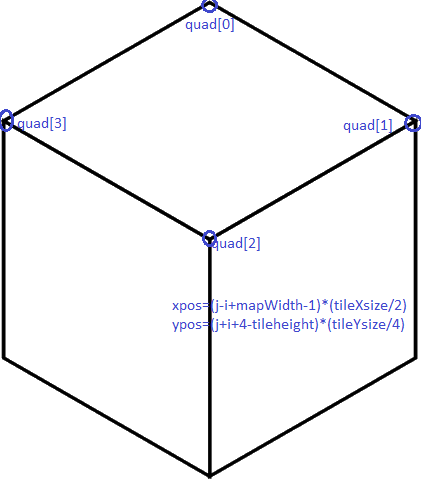
\includegraphics[]{images/carre_iso.png}
\centering
\caption{Schema calcul position isometrique}
\label{fig:img3}
\end{figure}

                quad[0].position = sf::Vector2f(xpos + tileXsize/2     , ypos + tileYsize/2    );
                \\quad[1].position = sf::Vector2f(xpos + tileXsize     , ypos + 3*(tileYsize/4)     );
                \\quad[2].position = sf::Vector2f(xpos + tileXsize/2   , ypos + tileYsize         );
                \\quad[3].position = sf::Vector2f(xpos                 , ypos + 3*(tileYsize/4)   );
\\
\\
    \item \textbf{La classe TurnDisplay:} La classe TurnDisplay est 
    constituée d'un constructeur qui génère un objet TurnDisplay pour un tour (turn) donné. 
    Il possède la réference à ce tour,
    une liste de tilesets et une liste de drawobjects vide.
    Sa fonction initRender appelle 
    les fonctions d'une instance de DrawObject 
    et les append à sa liste de drawobjects. 
    \\
    Pour les personnages, on fait un tableau à 2 dimensions pour
    stocker chaque sprites de l'animation des personnages.
\end{itemize}

\begin{figure}[H]
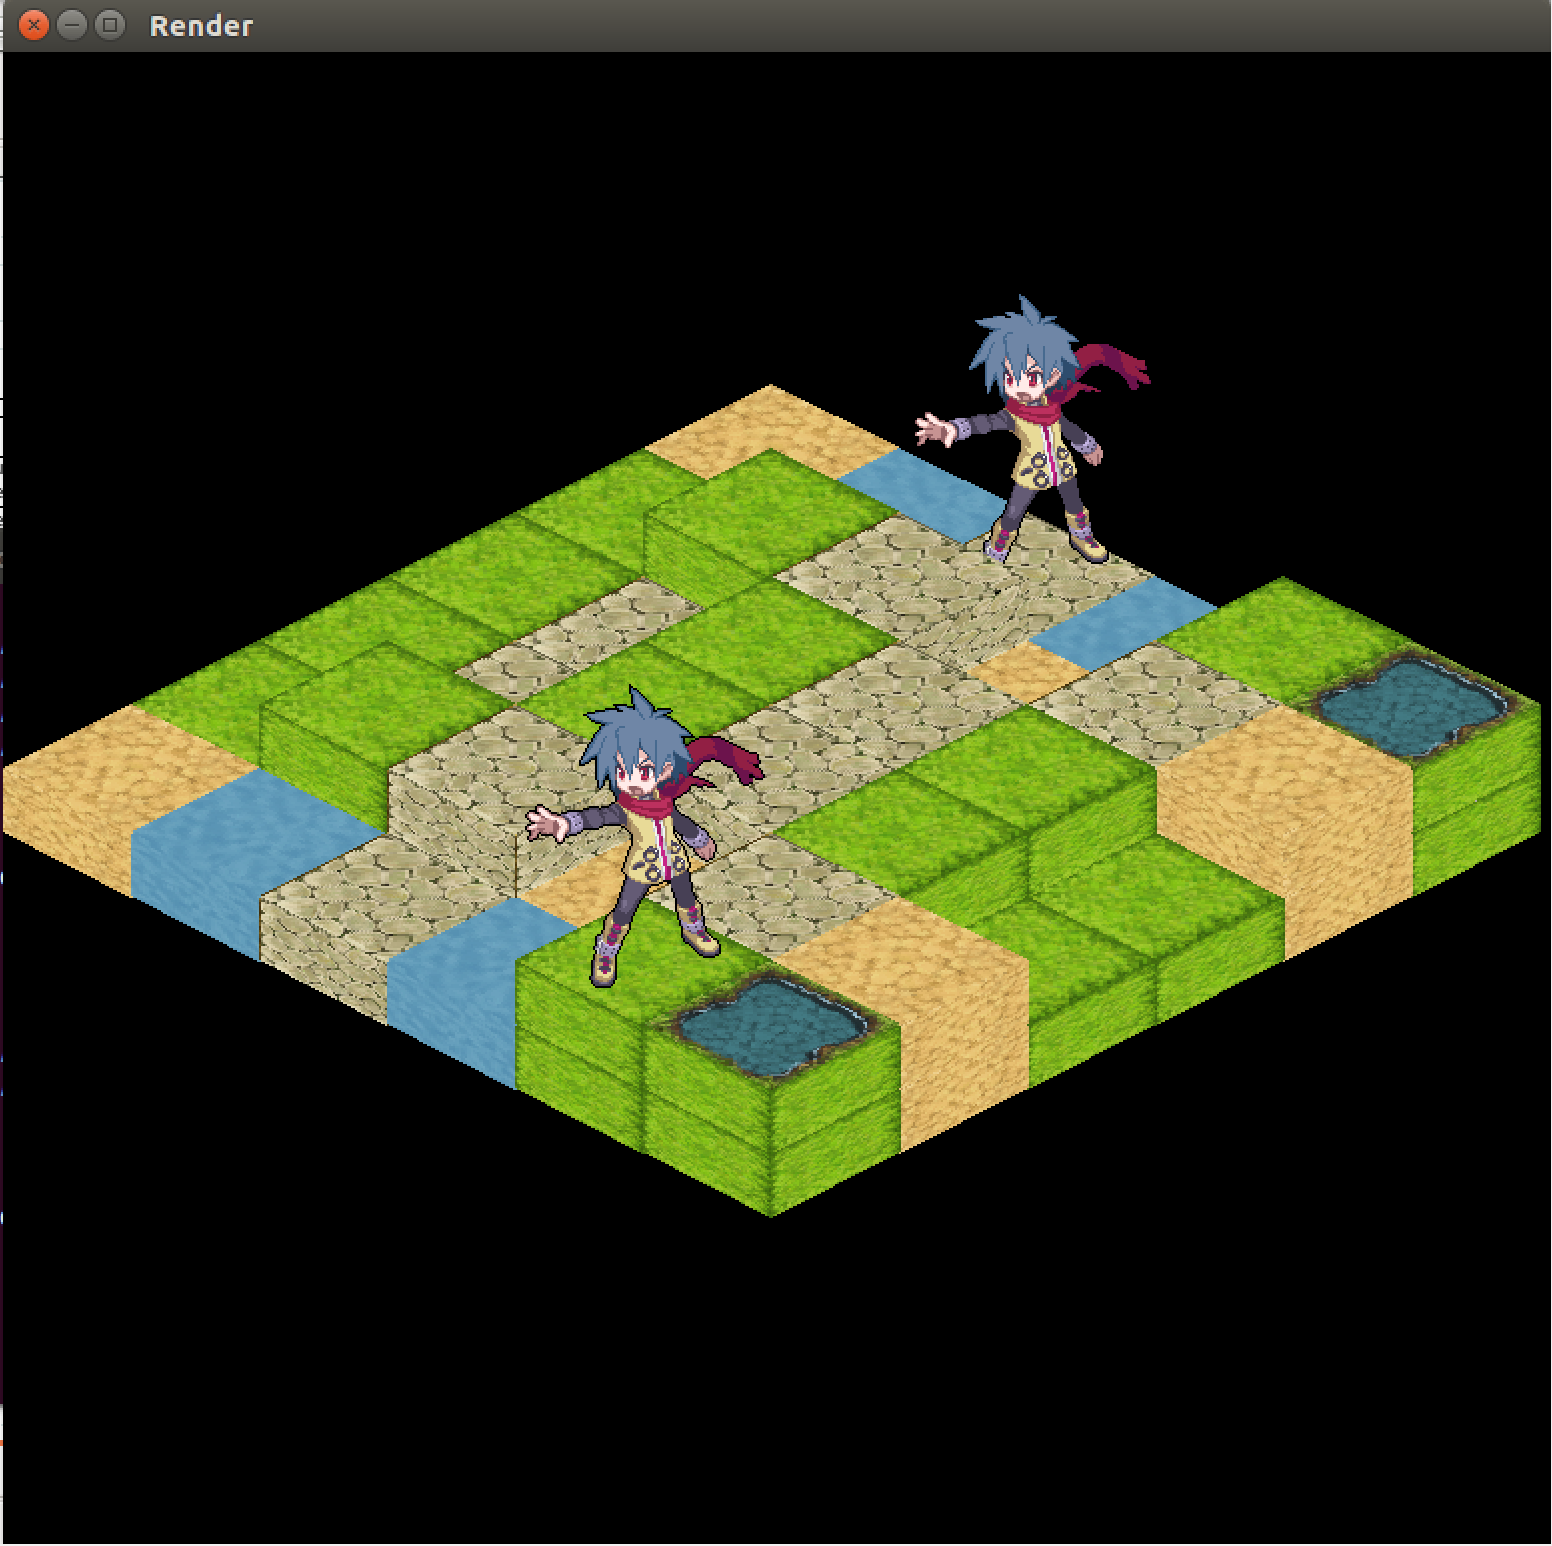
\includegraphics[width=\linewidth]{images/RenderPreview.png}
\centering
\caption{Aperçu du rendu d'un etat de jeu}
\label{fig:img3}
\end{figure}

\begin{figure}[H]
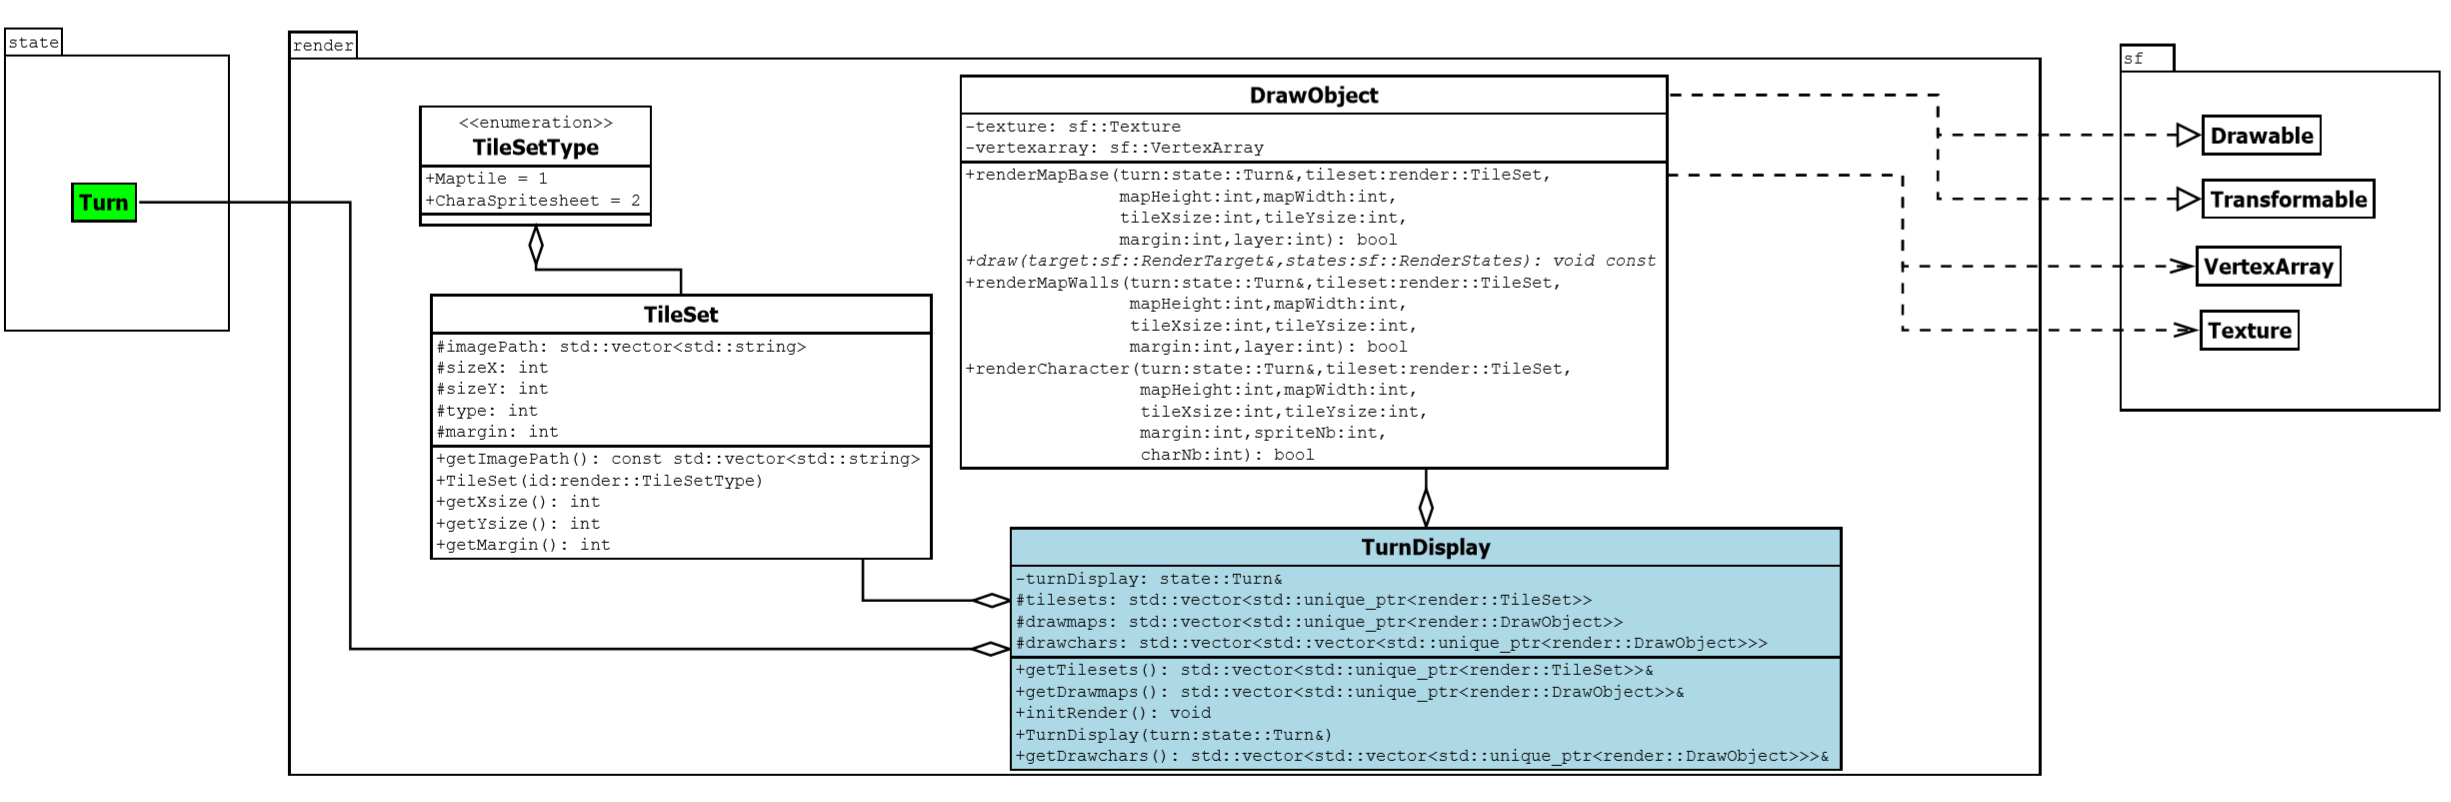
\includegraphics[width=\linewidth]{images/renderdia.png}
\centering
\caption{Aperçu de render.dia}
\label{fig:img3}
\end{figure}
